% Compile from the repository root with:
%   xelatex -interaction=nonstopmode report/TRYOPS_MLOPS_FINAL_REPORT_EN.tex
% or compile from report/; the graphic paths below support both locations.
\documentclass[12pt,a4paper,oneside]{report}

\usepackage[a4paper,top=2.5cm,bottom=2.5cm,left=2.8cm,right=2.2cm]{geometry}
\usepackage[T1]{fontenc}
\usepackage[utf8]{inputenc}
\usepackage{lmodern}
\usepackage{graphicx}
\usepackage{xcolor}
\usepackage{array}
\usepackage{booktabs}
\usepackage{longtable}
\usepackage{tabularx}
\usepackage{enumitem}
\usepackage{fancyhdr}
\usepackage{titlesec}
\usepackage{hyperref}
\usepackage{listings}
\usepackage{tikz}
\usepackage{float}
\usepackage{caption}
\usetikzlibrary{arrows.meta,positioning,fit,shapes.geometric,calc}

\graphicspath{
  {./}
  {report/assets/}
  {assets/}
}

\definecolor{TryOpsNavy}{HTML}{111827}
\definecolor{TryOpsInk}{HTML}{1F2937}
\definecolor{TryOpsBlue}{HTML}{2563EB}
\definecolor{TryOpsTeal}{HTML}{0F766E}
\definecolor{TryOpsGold}{HTML}{B45309}
\definecolor{TryOpsRed}{HTML}{B91C1C}
\definecolor{TryOpsSlate}{HTML}{475569}
\definecolor{TryOpsMist}{HTML}{F8FAFC}
\definecolor{TryOpsLine}{HTML}{CBD5E1}
\definecolor{CodeBg}{HTML}{F8FAFC}

\hypersetup{
  colorlinks=true,
  linkcolor=TryOpsBlue,
  urlcolor=TryOpsTeal,
  citecolor=TryOpsBlue,
  pdftitle={TryOps: Enterprise MLOps for Governed VTON and LLM Serving},
  pdfauthor={Nguyen Tran Nhat Trung, Hoang Minh Thai, Pham Hai Dang}
}

\pagestyle{fancy}
\fancyhf{}
\lhead{\small TryOps MLOps}
\rhead{\small Group1.CS317}
\cfoot{\thepage}
\setlength{\headheight}{14pt}
\renewcommand{\headrulewidth}{0.4pt}

\titleformat{\chapter}
  {\normalfont\huge\bfseries\color{TryOpsNavy}}
  {\thechapter.}{0.8em}{}
\titleformat{\section}
  {\normalfont\Large\bfseries\color{TryOpsNavy}}
  {\thesection}{0.7em}{}
\titleformat{\subsection}
  {\normalfont\large\bfseries\color{TryOpsNavy}}
  {\thesubsection}{0.6em}{}

\setlist[itemize]{leftmargin=1.1cm,itemsep=0.25em,topsep=0.25em}
\setlist[enumerate]{leftmargin=1.1cm,itemsep=0.25em,topsep=0.25em}
\renewcommand{\arraystretch}{1.22}
\setlength{\parindent}{0pt}
\setlength{\parskip}{0.55em}

\newcommand{\code}[1]{\texttt{\detokenize{#1}}}
\newcommand{\reporttitle}{TryOps: Enterprise MLOps for Governed Virtual Try-On and LLM Serving}
\newcommand{\reportsubtitle}{Governance Gates, Native Control Plane, Model Serving, and Production Observability}

\lstdefinestyle{tryopscode}{
  basicstyle=\small\ttfamily,
  backgroundcolor=\color{CodeBg},
  frame=single,
  rulecolor=\color{TryOpsLine},
  breaklines=true,
  columns=fullflexible,
  keepspaces=true,
  showstringspaces=false,
  tabsize=2
}
\lstset{style=tryopscode}

\newcommand{\pill}[2]{%
  \tikz[baseline=-0.55ex]\node[
    fill=#1!10,
    draw=#1!35,
    text=#1,
    rounded corners=3pt,
    inner xsep=6pt,
    inner ysep=2.8pt
  ]{\scriptsize\bfseries #2};%
}

\newcommand{\metric}[2][TryOpsBlue]{\textbf{\color{#1}#2}}

\newcommand{\metriccard}[4][TryOpsBlue]{%
  \fcolorbox{#1!35}{#1!7}{%
    \begin{minipage}[t]{#2}
      \centering
      {\scriptsize\bfseries\color{TryOpsSlate}#3\par}
      \vspace{0.10em}
      {\Large\bfseries\color{#1}#4\par}
    \end{minipage}%
  }%
}

\newcommand{\techlogo}[2]{%
  \begin{minipage}[t]{1.52cm}
    \centering
    \includegraphics[height=0.50cm,width=1.36cm,keepaspectratio]{#1}\\[-0.03cm]
    {\tiny #2}
  \end{minipage}\hspace{0.06cm}%
}

\newcommand{\techchip}[2][TryOpsSlate]{%
  \tikz[baseline=(n.base)]\node[
    fill=#1!8,
    draw=#1!35,
    text=TryOpsInk,
    rounded corners=2pt,
    inner xsep=4.5pt,
    inner ysep=2pt
  ](n){\scriptsize\bfseries #2};\hspace{0.08cm}%
}

\newcommand{\infobox}[2]{%
  \vspace{0.3em}
  \noindent
  \fcolorbox{TryOpsBlue!25}{TryOpsBlue!5}{%
    \begin{minipage}{0.96\linewidth}
      \textbf{\color{TryOpsNavy}#1}\par
      #2
    \end{minipage}
  }
  \vspace{0.3em}
}

\newcommand{\screenshotfig}[2]{%
  \begin{figure}[H]
    \centering
    \includegraphics[width=\linewidth]{#1}
    \caption[#2]{#2.}
  \end{figure}
}

\begin{document}

% ---------------------------------------------------------------------------
% Cover
% ---------------------------------------------------------------------------
\begin{titlepage}
  \thispagestyle{empty}
  \centering
  \begin{tikzpicture}[remember picture,overlay]
    \draw[line width=1.7pt,color=TryOpsBlue]
      ([xshift=1.35cm,yshift=-1.35cm]current page.north west)
      rectangle
      ([xshift=-1.35cm,yshift=1.35cm]current page.south east);
    \draw[line width=0.65pt,color=TryOpsBlue]
      ([xshift=1.50cm,yshift=-1.50cm]current page.north west)
      rectangle
      ([xshift=-1.50cm,yshift=1.50cm]current page.south east);
    \draw[line width=0.55pt,color=TryOpsLine]
      ([xshift=1.78cm,yshift=-1.78cm]current page.north west)
      -- ++(1.45cm,0) arc[start angle=90,end angle=0,radius=0.45cm] -- ++(0,-1.45cm);
    \draw[line width=0.55pt,color=TryOpsLine]
      ([xshift=-1.78cm,yshift=1.78cm]current page.south east)
      -- ++(-1.45cm,0) arc[start angle=-90,end angle=-180,radius=0.45cm] -- ++(0,1.45cm);
    \draw[line width=0.35pt,color=TryOpsLine]
      ([xshift=2.02cm,yshift=-2.02cm]current page.north west)
      -- ++(0.95cm,0) arc[start angle=90,end angle=0,radius=0.28cm] -- ++(0,-0.95cm);
    \draw[line width=0.35pt,color=TryOpsLine]
      ([xshift=-2.02cm,yshift=2.02cm]current page.south east)
      -- ++(-0.95cm,0) arc[start angle=-90,end angle=-180,radius=0.28cm] -- ++(0,0.95cm);
  \end{tikzpicture}

  \vspace*{-0.25cm}
  {\bfseries\Large VIETNAM NATIONAL UNIVERSITY, HO CHI MINH CITY\par}
  \vspace{0.22cm}
  {\bfseries\Large UNIVERSITY OF INFORMATION TECHNOLOGY\par}
  \vspace{0.22cm}
  {\bfseries\large FACULTY OF COMPUTER SCIENCE\par}

  \vspace{0.72cm}
  
\includegraphics[height=3.1cm,trim=0 305 0 0,clip]{uit-emblem.png}\par
  \vspace{0.05cm}
  % {\Huge\bfseries\color{TryOpsBlue}UIT-HCM\par}

  \vspace{0.72cm}
  {\bfseries\large COURSE\par}
  \vspace{0.18cm}
  {\large CS317.Q22 -- DEVELOPMENT AND OPERATION OF MACHINE LEARNING SYSTEMS\par}

  \vspace{0.72cm}
  {\bfseries\large FINAL PROJECT REPORT\par}
  \vspace{0.28cm}
  \begin{minipage}{0.84\textwidth}
    \centering
    {\bfseries\Large\color{TryOpsNavy}\reporttitle\par}
  \end{minipage}
  \vspace{0.26cm}

  {\normalsize\textbf{Repository:} \href{https://github.com/trungdangtapcode/TryOps-TryON-MLOps}{github.com/trungdangtapcode/TryOps-TryON-MLOps}\par}

  \vspace{0.58cm}
  \begin{tabular}{>{\bfseries}p{4.2cm}p{7.2cm}}
    Instructor: & MSc. Do Van Tien \\
    Teaching Assistant: & Le Tran Trong Khiem \\
  \end{tabular}

  \vspace{0.58cm}
  \begin{tabular}{>{\bfseries}p{2.1cm}p{6.4cm}p{2.9cm}}
    Students: & Nguyen Tran Nhat Trung & 23521684 \\
              & Hoang Minh Thai & 23521414 \\
              & Pham Hai Dang & 23520233 \\
  \end{tabular}

  \vfill
  {\large Ho Chi Minh City, July 2026\par}
\end{titlepage}

\pagenumbering{roman}

\chapter*{Executive Summary}
\addcontentsline{toc}{chapter}{Executive Summary}

TryOps is an enterprise-oriented MLOps platform built around two demanding AI workloads: Virtual Try-On (VTON) and Large Language Model (LLM) serving. The project focuses on the operational system around model changes: data and artifact tracking, configured inference endpoints, account and quota control, asynchronous jobs, policy gates, model registry records, observability, incident response, rollback posture, and a clear line between production behavior and test-only diagnostics.

The system is composed of four main layers. The product layer is a React/Vite console that supports login, account/workspace context, LLM requests, VTON upload and job tracking, model registry, governance, dashboards, and history. The edge layer is a Rust Axum gateway responsible for authentication, proxying, request limits, quota admission, guardrail dispatch, static serving, and Prometheus metrics. The workflow layer is a FastAPI backend that owns product APIs, VTON job orchestration, artifact metadata, evaluation, history, account state, and governance views. The inference and control-plane layer includes a host-side FASHN VTON router and workers, an OpenAI-compatible LLM endpoint, Go services, and C++ native tools for policy, metrics, SLO checks, supply-chain records, cache, energy, and evaluation.

The strongest engineering decision in TryOps is the fail-closed model-serving boundary. Production-local defaults require configured VTON and LLM endpoints. If those endpoints are unavailable, the system returns explicit operational errors. This keeps production behavior auditable and separates end-user inference from contract tests.

The current implementation supports a developer-local product stack with Postgres, Valkey, MinIO, MLflow, Keycloak, FastAPI, Rust Gateway, Go guardrail, Prometheus, Grafana, Loki, Tempo, OpenTelemetry Collector, and a host-side FASHN VTON router. The report includes product screenshots for the UI, workspace quota, running VTON jobs, Keycloak, MinIO, MLflow, Grafana, log drilldown, and architecture diagrams.

\textbf{Keywords:} MLOps, Virtual Try-On, FASHN VTON, LLM Serving, vLLM, OpenAI-compatible API, Rust Gateway, FastAPI, Go, C++, Prometheus, Grafana, Loki, MLflow, MinIO, Keycloak, governance, policy gates.

\tableofcontents
\listoffigures
\clearpage
\pagenumbering{arabic}

% ---------------------------------------------------------------------------
\chapter{Introduction}
% ---------------------------------------------------------------------------

\section{Motivation}

Many ML applications can produce one impressive screenshot. Production ML systems require much more. A production-grade ML application must answer operational questions that are invisible in a notebook:

\begin{itemize}
  \item Which data, model weights, code version, configuration, and hardware produced an output?
  \item Can a bad candidate model be blocked before users see it?
  \item Does the system report an operational error when a configured model endpoint is unavailable?
  \item Can each workspace be controlled by quota, rate limits, and concurrency limits?
  \item Can operators debug failures through metrics, logs, traces, job IDs, and request IDs?
  \item Can a release be rolled back and explained to a risk reviewer?
\end{itemize}

TryOps was designed to answer these questions. The chosen workloads are deliberately different. VTON is visual, GPU-heavy, privacy-sensitive, artifact-oriented, and hard to evaluate because visual defects are often qualitative. LLM serving is latency-sensitive, token-cost-sensitive, guardrail-sensitive, and vulnerable to prompt injection and output policy issues. A platform that can operate both workloads behind the same governance spine demonstrates MLOps thinking beyond a single workload.

\section{Project Objectives}

The project objective is to build a working MLOps platform that can serve production model workloads while preserving traceability, observability, quota, and governance.

Concrete objectives:

\begin{enumerate}
  \item Build a TryOps Console for end users, operators, and reviewers.
  \item Use a Rust gateway as the production-facing edge boundary.
  \item Use FastAPI as the product workflow backend and model adapter layer.
  \item Run VTON through a host-side FASHN VTON serving path.
  \item Support LLM inference through an OpenAI-compatible endpoint, including self-hosted vLLM or a managed API.
  \item Integrate Keycloak for OIDC login and workspace identity.
  \item Integrate Postgres, Valkey, MinIO, and MLflow for product data, counters, objects, and experiment tracking.
  \item Integrate Prometheus, Grafana, Loki, Tempo, and OpenTelemetry for observability.
  \item Implement model governance through policy gates, supply-chain records, model cards, data cards, and promotion records.
  \item Keep test and evaluation utilities separate from production model behavior.
\end{enumerate}

\section{Scope}

\begin{longtable}{p{3.2cm}p{5.9cm}p{5.9cm}}
\toprule
\textbf{Area} & \textbf{Included in the project} & \textbf{Scoped or future work} \\
\midrule
Product & TryOps Console, LLM Playground, VTON Studio, Account, Registry, Governance, Dashboard, History & Additional accessibility polish, export workflows, and more operator click-through actions \\
VTON & FASHN VTON router, GPU workers, image upload, async jobs, artifact output, metrics & Larger human preference study and broader production model zoo \\
LLM & OpenAI-compatible endpoint, OpenAI/vLLM configuration, guardrails, quota & Full live vLLM benchmark depends on the active workspace and GPU availability \\
MLOps & MLflow, MinIO, promotion records, model/data cards, policy gates & Full production KServe/Kubeflow deployment profile \\
Observability & Prometheus, Grafana, Loki, Tempo, OTel bridge, structured logs & Complete GPU/process exporters for every shared-datacenter variant \\
Security & Keycloak, gateway auth, quota, guardrails, supply-chain records & External Secrets/Vault production synchronization \\
Networking & Developer-local port map and shared-datacenter plan & Final ingress/hardening profile for a multi-tenant data center \\
\bottomrule
\end{longtable}

\section{Main Contributions}

\begin{itemize}
  \item A repeatable local deployment path for the full product stack.
  \item A native-first production boundary: Rust at the edge, Go for services/controllers/load tools, C++ for native tools, and Python for ML workflows.
  \item A VTON serving abstraction: the API calls a stable serving endpoint, while the router hides worker count, GPU mapping, sockets, and per-worker metrics.
  \item An LLM adapter using an OpenAI-compatible API and explicit endpoint-error handling.
  \item A configured observability stack with Grafana dashboards, Loki logs, Tempo traces, Prometheus metrics, and structured job/request logs.
  \item A governance pipeline containing policy gates, supply-chain records, dependency locks, model scans, provenance, and promotion lifecycle records.
\end{itemize}

\section{Technology Stack}

\begin{figure}[H]
  \centering
  \small
  \setlength{\tabcolsep}{5pt}
  \renewcommand{\arraystretch}{1.5}
  \begin{tabularx}{\linewidth}{>{\raggedright\arraybackslash\bfseries\color{TryOpsNavy}}p{2.8cm}X}
    Product UI &
      \techlogo{logos/react.png}{React}
      \techlogo{logos/typescript.png}{TypeScript}
      \techlogo{logos/vite.png}{Vite}
      \techlogo{logos/lucide.png}{Lucide}
      \techlogo{logos/tailwind.png}{Tailwind} \\
    API and Native Runtime &
      \techlogo{logos/python.png}{Python}
      \techlogo{logos/fastapi.png}{FastAPI}
      \techlogo{logos/rust.png}{Rust}
      \techlogo{logos/go.png}{Go}
      \techlogo{logos/cplusplus.png}{C++}
      \techlogo{logos/docker.png}{Docker} \\
    Data, Identity, and Governance &
      \techlogo{logos/postgresql.png}{Postgres}
      \techlogo{logos/valkey.png}{Valkey}
      \techlogo{logos/minio.png}{MinIO}
      \techlogo{logos/mlflow.png}{MLflow}
      \techlogo{logos/dvc.png}{DVC}
      \techlogo{logos/keycloak.png}{Keycloak} \\
    Model Serving and AI Libraries &
      \techlogo{logos/pytorch.png}{PyTorch}
      \techlogo{logos/huggingface.png}{HF Hub}
      \techlogo{logos/fashn.png}{FASHN VTON}
      \techlogo{logos/openai.png}{OpenAI API}
      \techlogo{logos/vllm.png}{vLLM} \\
    Observability and Operations &
      \techlogo{logos/prometheus.png}{Prometheus}
      \techlogo{logos/grafana.png}{Grafana}
      \techlogo{logos/loki.png}{Loki}
      \techlogo{logos/tempo.png}{Tempo}
      \techlogo{logos/opentelemetry.png}{OTel}
      \techlogo{logos/alertmanager.png}{Alertmanager} \\
  \end{tabularx}
  \caption{TryOps technology stack grouped by product layer.}
\end{figure}

% ---------------------------------------------------------------------------
\chapter{Background and Engineering Principles}
% ---------------------------------------------------------------------------

\section{MLOps Requirements}

MLOps is the discipline of moving machine learning from research to controlled operation. For this project, the important MLOps requirements are:

\begin{itemize}
  \item Versioning for data, code, configuration, and model artifacts.
  \item Experiment tracking and artifact storage.
  \item Automated evaluation before promotion.
  \item Model registry with lifecycle states: candidate, challenger, champion, rejected, archived.
  \item CI/CD and policy gates.
  \item Observability for metrics, logs, traces, drift, quality, and cost.
  \item Security, quota, guardrails, and rollback.
\end{itemize}

TryOps implements these through MLflow, MinIO, Postgres, Valkey, local artifacts, generated reports, repeatable operational targets, native policy/evaluation tools, and Grafana/Loki/Tempo dashboards.

\section{Virtual Try-On}

Virtual Try-On accepts a person image and a garment image, then generates an image of the person wearing that garment. It is operationally difficult because:

\begin{itemize}
  \item The output is visual, and failures may be geometric distortion, identity drift, texture loss, incorrect pose, broken limbs, or artifacts at garment boundaries.
  \item GPU memory and latency can be large.
  \item Person images are privacy-sensitive.
  \item The system must preserve input, output, report, metrics, and lineage.
  \item The system must record whether an output came from the production VTON path or from evaluation code.
\end{itemize}

TryOps uses FASHN VTON v1.5 as the production-local VTON path. The public FASHN research note describes v1.5 as a maskless pixel-space virtual try-on model designed to preserve garment detail without requiring segmentation masks.\footnote{\url{https://fashn.ai/research/vton-1-5}} Evaluation image utilities may be kept for contract tests, but they are not enabled as the default end-user product path.

\section{LLM Serving}

LLM serving requires tracking latency, throughput, token counts, token cost, quota, cache effects, guardrail outcomes, and endpoint failures. TryOps standardizes LLM serving through an OpenAI-compatible API. The endpoint may be self-hosted or managed by a provider, but the production contract remains the same: user prompts are sent to a configured model endpoint, provider secrets are injected through secure runtime configuration, and endpoint failures are surfaced through the product and observability stack.

% ---------------------------------------------------------------------------
\chapter{Requirements Analysis}
% ---------------------------------------------------------------------------

\section{Actors}

\begin{longtable}{p{4.2cm}p{10.5cm}}
\toprule
\textbf{Actor} & \textbf{Needs} \\
\midrule
End user & Login, upload images, run try-on, inspect status, open results \\
ML engineer & Run benchmark jobs, compare candidates, inspect generated evaluation reports \\
Platform engineer & Operate the stack, inspect logs/metrics/traces, manage model endpoints and ports \\
Risk reviewer & Inspect model cards, data cards, policy gates, supply-chain records, and lineage \\
Admin/operator & Monitor quota, accounts, registry state, incidents, and rollback records \\
Evaluator/instructor & Verify system behavior through code, commands, dashboards, artifacts, and reports \\
\bottomrule
\end{longtable}

\section{Functional Requirements}

\begin{enumerate}
  \item Authenticate users with Keycloak/OIDC and bootstrap a workspace.
  \item Upload person and garment images.
  \item Submit VTON jobs asynchronously.
  \item Poll job status and open output artifacts.
  \item Send LLM prompts to a configured endpoint.
  \item Apply workspace quota and VTON concurrency limits.
  \item Store request history, job history, artifact metadata, and feedback.
  \item Provide dashboard rollups for operators.
  \item Provide governance and model registry views.
  \item Support promotion records, rejection records, and rollback records.
  \item Export logs, metrics, and traces for debugging.
\end{enumerate}

\section{Non-Functional Requirements}

\begin{longtable}{p{4.2cm}p{10.5cm}}
\toprule
\textbf{Requirement} & \textbf{TryOps design response} \\
\midrule
Configured model execution & Production model endpoints are required for end-user workflows \\
Fail-closed model serving & LLM and VTON adapters return errors if configured endpoints fail \\
Reproducibility & Make targets, artifacts, run context, dependency locks, and generated reports \\
Security & Keycloak, Rust gateway auth, development authentication shortcuts disabled by default \\
Privacy & Structured logs avoid raw prompt/image content and use job/request IDs \\
Observability & Prometheus, Grafana, Loki, Tempo, OpenTelemetry, structured logs \\
Scalability & FASHN router hides multiple GPU workers behind one endpoint \\
Shared datacenter fit & Plan to expose only necessary ports and keep internal services private \\
Operability & Repeatable startup/shutdown workflows, smoke tests, health checks, dashboards \\
\bottomrule
\end{longtable}

\section{Production vs Diagnostics Boundary}

\begin{longtable}{p{3.4cm}p{5.8cm}p{5.8cm}}
\toprule
\textbf{Component} & \textbf{Production path} & \textbf{Test/evaluation utilities} \\
\midrule
VTON & FASHN router through the configured VTON serving endpoint & Overlay/image utilities only when explicitly enabled for tests \\
LLM & OpenAI-compatible model endpoint & Request/response harnesses only for adapter checks \\
Semantic cache & Controlled and observable feature & Disabled by default in production-safety config \\
API keys & OIDC/JWT and provider secrets & Static development key disabled by default \\
Worker ports & Hidden behind router & Direct worker port only for debugging \\
\bottomrule
\end{longtable}

% ---------------------------------------------------------------------------
\chapter{System Architecture}
% ---------------------------------------------------------------------------

\section{Architecture Overview}

\begin{figure}[H]
\centering
\scriptsize
\resizebox{\linewidth}{!}{%
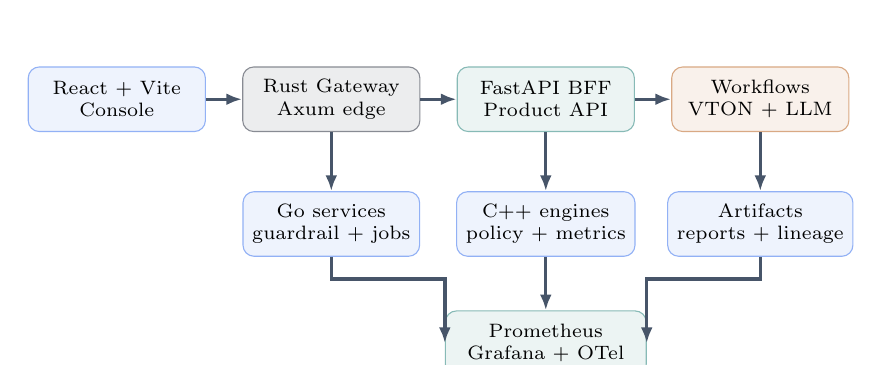
\begin{tikzpicture}[
  node distance=0.38cm and 0.46cm,
  every node/.style={font=\scriptsize},
  boundary/.style={draw=#1!50, fill=#1!8, rounded corners=4pt, minimum width=2.25cm, minimum height=0.82cm, align=center},
  arrow/.style={-{Latex[length=2mm]}, very thick, color=TryOpsSlate}
]
\node[boundary=TryOpsBlue] (web) {React + Vite\\Console};
\node[boundary=TryOpsNavy, right=of web] (gateway) {Rust Gateway\\Axum edge};
\node[boundary=TryOpsTeal, right=of gateway] (api) {FastAPI BFF\\Product API};
\node[boundary=TryOpsGold, right=of api] (workflows) {Workflows\\VTON + LLM};

\node[boundary=TryOpsBlue, minimum width=2.05cm, below=0.75cm of gateway] (go) {Go services\\guardrail + jobs};
\node[boundary=TryOpsBlue, minimum width=2.05cm, below=0.75cm of api] (cpp) {C++ engines\\policy + metrics};
\node[boundary=TryOpsBlue, minimum width=2.05cm, below=0.75cm of workflows] (store) {Artifacts\\reports + lineage};
\node[boundary=TryOpsTeal, minimum width=2.55cm, below=0.68cm of cpp] (obs) {Prometheus\\Grafana + OTel};

\draw[arrow] (web) -- (gateway);
\draw[arrow] (gateway) -- (api);
\draw[arrow] (api) -- (workflows);
\draw[arrow] (gateway) -- (go);
\draw[arrow] (api) -- (cpp);
\draw[arrow] (workflows) -- (store);
\draw[arrow] (go.south) -- ++(0,-0.28) -| (obs.west);
\draw[arrow] (cpp.south) -- (obs.north);
\draw[arrow] (store.south) -- ++(0,-0.28) -| (obs.east);
\end{tikzpicture}%
}

\vspace{0.45em}
\begin{minipage}[t]{0.48\linewidth}
\fcolorbox{TryOpsBlue!22}{TryOpsBlue!5}{%
  \begin{minipage}{0.94\linewidth}
  \textbf{Compiled production boundary}\par
  Rust fronts \code{/api/*}; Go owns sidecars, controller-style services, and native drivers; C++ supports native tools.
  \end{minipage}}
\end{minipage}\hfill
\begin{minipage}[t]{0.48\linewidth}
\fcolorbox{TryOpsTeal!22}{TryOpsTeal!5}{%
  \begin{minipage}{0.94\linewidth}
  \textbf{Python role}\par
  Python coordinates ML workflows and product APIs, while risk-critical decisions are mirrored or moved into native tools.
  \end{minipage}}
\end{minipage}
\caption{Product boundary architecture diagram.}
\end{figure}

\begin{figure}[H]
\centering
\scriptsize
\resizebox{\linewidth}{!}{%
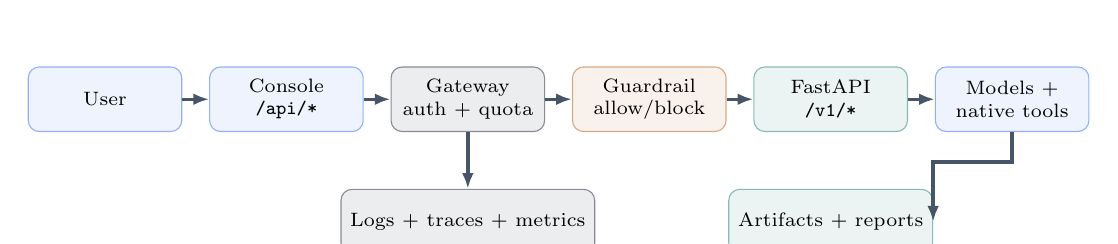
\begin{tikzpicture}[
  node distance=0.28cm and 0.34cm,
  every node/.style={font=\scriptsize},
  flow/.style={draw=#1!50, fill=#1!8, rounded corners=4pt, minimum width=1.95cm, minimum height=0.82cm, align=center},
  arrow/.style={-{Latex[length=2mm]}, very thick, color=TryOpsSlate}
]
\node[flow=TryOpsBlue] (user) {User};
\node[flow=TryOpsBlue, right=of user] (console) {Console\\\code{/api/*}};
\node[flow=TryOpsNavy, right=of console] (gateway) {Gateway\\auth + quota};
\node[flow=TryOpsGold, right=of gateway] (guardrail) {Guardrail\\allow/block};
\node[flow=TryOpsTeal, right=of guardrail] (api) {FastAPI\\\code{/v1/*}};
\node[flow=TryOpsBlue, right=of api] (models) {Models +\\native tools};

\node[flow=TryOpsTeal, minimum width=2.35cm, below=0.72cm of api] (artifacts) {Artifacts + reports};
\node[flow=TryOpsNavy, minimum width=2.35cm, below=0.72cm of gateway] (obs) {Logs + traces + metrics};

\draw[arrow] (user) -- (console);
\draw[arrow] (console) -- (gateway);
\draw[arrow] (gateway) -- (guardrail);
\draw[arrow] (guardrail) -- (api);
\draw[arrow] (api) -- (models);
\draw[arrow] (models.south) -- ++(0,-0.38) -| (artifacts.east);
\draw[arrow] (gateway.south) -- (obs.north);
\end{tikzpicture}%
}

\vspace{0.45em}
\begin{tabularx}{\linewidth}{>{\raggedright\arraybackslash}X>{\raggedright\arraybackslash}X}
\toprule
\textbf{Edge responsibilities} & \textbf{Workflow responsibilities} \\
\midrule
API-key and token checks, request IDs, rate and body limits, quota admission, semantic-cache admission, edge guardrail calls, metrics, and proxying. &
VTON, LLM, evaluation, governance, promotion, rollback, and artifact writes under reproducible run context. \\
\bottomrule
\end{tabularx}
\caption{Request flow from console entry point to model output and audit records.}
\end{figure}

\begin{figure}[H]
\centering
\scriptsize
\resizebox{\linewidth}{!}{%
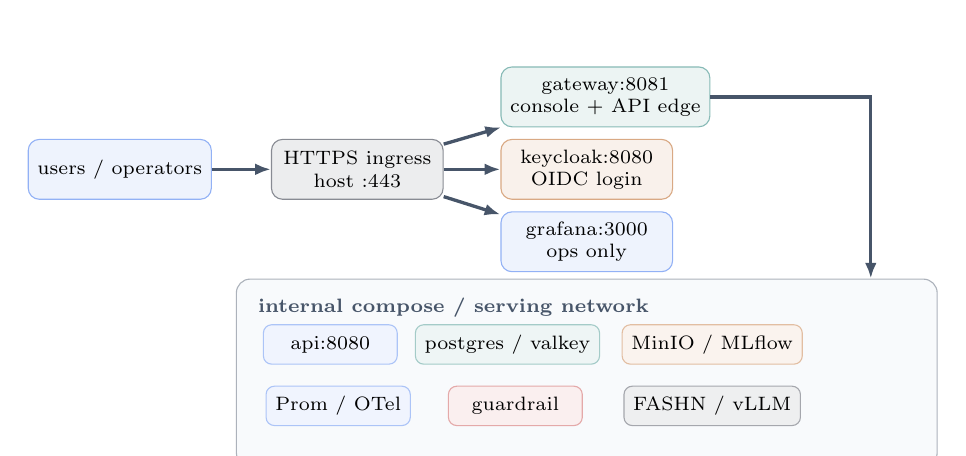
\begin{tikzpicture}[
  node distance=0.35cm,
  every node/.style={font=\scriptsize},
  port/.style={draw=#1!50, fill=#1!8, rounded corners=4pt, minimum width=2.18cm, minimum height=0.76cm, align=center},
  tinyport/.style={draw=#1!38, fill=#1!7, rounded corners=3pt, minimum width=1.70cm, minimum height=0.50cm, align=center},
  arrow/.style={-{Latex[length=2mm]}, very thick, color=TryOpsSlate}
]
\node[port=TryOpsBlue] (users) {users / operators};
\node[port=TryOpsNavy, right=0.75cm of users] (ingress) {HTTPS ingress\\host :443};

\node[port=TryOpsTeal, right=0.72cm of ingress, yshift=0.92cm] (gateway) {gateway:8081\\console + API edge};
\node[port=TryOpsGold, right=0.72cm of ingress] (keycloak) {keycloak:8080\\OIDC login};
\node[port=TryOpsBlue, right=0.72cm of ingress, yshift=-0.92cm] (grafana) {grafana:3000\\ops only};

\node[draw=TryOpsSlate!45, fill=TryOpsMist, rounded corners=5pt, minimum width=8.90cm, minimum height=2.38cm, align=center, below=1.00cm of keycloak] (internal) {};
\node[anchor=north west, text=TryOpsSlate] at ($(internal.north west)+(0.16,-0.12)$) {\bfseries internal compose / serving network};
\node[tinyport=TryOpsBlue] at ($(internal.west)+(1.20,0.36)$) {api:8080};
\node[tinyport=TryOpsTeal, minimum width=2.05cm] at ($(internal.west)+(3.45,0.36)$) {postgres / valkey};
\node[tinyport=TryOpsGold, minimum width=1.95cm] at ($(internal.west)+(6.05,0.36)$) {MinIO / MLflow};
\node[tinyport=TryOpsBlue] at ($(internal.west)+(1.30,-0.42)$) {Prom / OTel};
\node[tinyport=TryOpsRed] at ($(internal.west)+(3.55,-0.42)$) {guardrail};
\node[tinyport=TryOpsNavy, minimum width=2.20cm] at ($(internal.west)+(6.05,-0.42)$) {FASHN / vLLM};

\draw[arrow] (users) -- (ingress);
\draw[arrow] (ingress) -- (gateway);
\draw[arrow] (ingress) -- (keycloak);
\draw[arrow] (ingress) -- (grafana);
\draw[arrow] (gateway.east) -- ++(0.52,0) -| ($(internal.north east)+(-0.85,0)$);
\end{tikzpicture}%
}

\vspace{0.45em}
\begin{tabularx}{\linewidth}{>{\raggedright\arraybackslash}X>{\raggedright\arraybackslash}X}
\toprule
\textbf{Recommended shared-host surface} & \textbf{Developer-local exception} \\
\midrule
One TLS ingress routes to the gateway, Keycloak, and admin-restricted Grafana. FastAPI, databases, object stores, metrics backends, guardrail, and model endpoints stay private. &
\code{make app-up} exposes convenience ports for local debugging. That is not the shared-datacenter posture. \\
\bottomrule
\end{tabularx}
\caption{Recommended port surface for shared hosts.}
\end{figure}

\begin{figure}[H]
\centering
\small
\begin{tabularx}{\linewidth}{>{\raggedright\arraybackslash}X>{\raggedright\arraybackslash}X>{\raggedright\arraybackslash}X}
\toprule
\textbf{Observe} & \textbf{Recover} & \textbf{Govern} \\
\midrule
OpenTelemetry trace/log correlation; Prometheus metrics and Alertmanager routing; Grafana service, quality, cost, capacity, and energy panels. &
Rollback samples; chaos drills for GPU OOM, slow decode, corrupted weights, and poisoned candidates; C++ burn-rate logic for SRE-style paging. &
NIST AI RMF and OWASP LLM mapping; model-source pins, SBOM, scans, SafeTensors gate; signed PR and registry-webhook release triggers. \\
\bottomrule
\end{tabularx}

\vspace{0.55em}
\fcolorbox{TryOpsBlue!22}{TryOpsBlue!5}{%
  \begin{minipage}{0.92\linewidth}
  \textbf{Why it matters.} The platform does not only produce model outputs; it produces operational records that an evaluator, SRE, or risk reviewer can inspect.
  \end{minipage}}
\caption{Observability, reliability, and governance summary.}
\end{figure}

\section{Layered Architecture}

\begin{figure}[H]
\centering
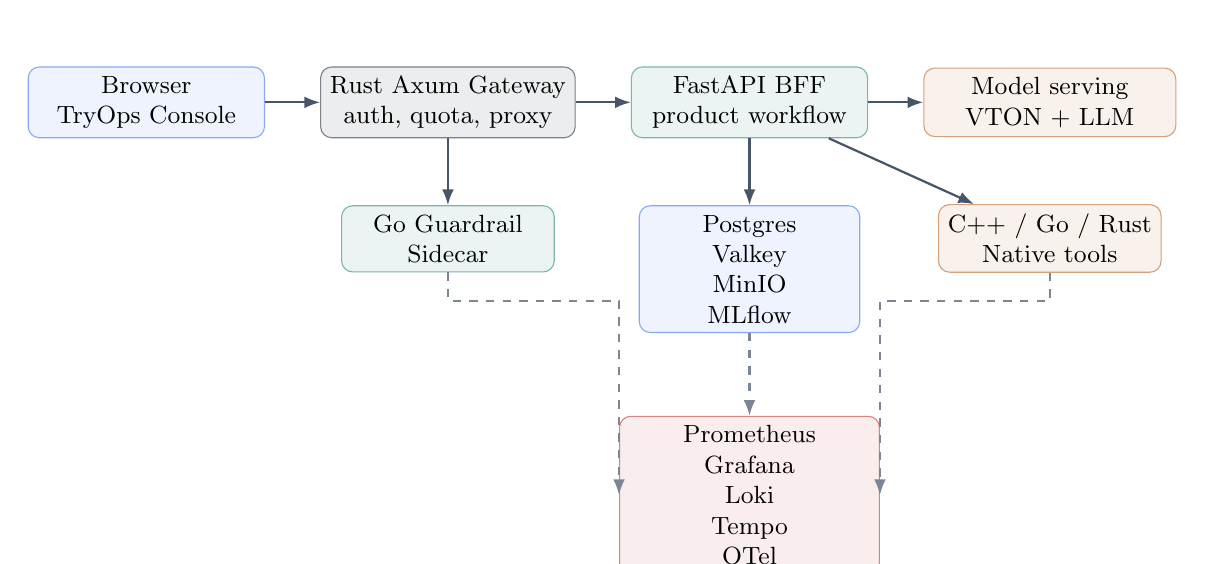
\begin{tikzpicture}[
  node distance=0.85cm and 0.7cm,
  box/.style={draw=#1!55, fill=#1!8, rounded corners=4pt, minimum height=0.84cm, align=center, font=\small},
  arrow/.style={-{Latex[length=2mm]}, thick, color=TryOpsSlate},
  telemetry/.style={-{Latex[length=2mm]}, thick, dashed, color=TryOpsSlate!72}
]
\node[box=TryOpsBlue, minimum width=3.0cm] (user) {Browser\\TryOps Console};
\node[box=TryOpsNavy, minimum width=3.2cm, right=of user] (gateway) {Rust Axum Gateway\\auth, quota, proxy};
\node[box=TryOpsTeal, minimum width=3.0cm, right=of gateway] (api) {FastAPI BFF\\product workflow};
\node[box=TryOpsGold, minimum width=3.2cm, right=of api] (models) {Model serving\\VTON + LLM};

\node[box=TryOpsTeal, minimum width=2.7cm, below=of gateway] (guardrail) {Go Guardrail\\Sidecar};
\node[box=TryOpsBlue, minimum width=2.8cm, below=of api] (data) {Postgres\\Valkey\\MinIO\\MLflow};
\node[box=TryOpsGold, minimum width=2.8cm, below=of models] (native) {C++ / Go / Rust\\Native tools};
\node[box=TryOpsRed, minimum width=3.3cm, below=1.05cm of data] (obs) {Prometheus\\Grafana\\Loki\\Tempo\\OTel};

\draw[arrow] (user) -- (gateway);
\draw[arrow] (gateway) -- (api);
\draw[arrow] (api) -- (models);
\draw[arrow] (gateway) -- (guardrail);
\draw[arrow] (api) -- (data);
\draw[arrow] (api) -- (native);
\draw[telemetry] (guardrail.south) -- ++(0,-0.36) -| (obs.west);
\draw[telemetry] (data.south) -- (obs.north);
\draw[telemetry] (native.south) -- ++(0,-0.36) -| (obs.east);
\end{tikzpicture}
\caption{TryOps layered architecture.}
\end{figure}

\section{Frontend Layer}

The frontend is organized around product workflows rather than isolated examples. Its main capabilities include:

\begin{itemize}
  \item VTON image upload, garment/source/quality selection, and asynchronous job submission.
  \item Active, queued, completed, and failed job presentation.
  \item Recent VTON output gallery.
  \item LLM prompt workflow.
  \item Workspace quota and account state.
  \item Operator views for dashboards, governance, registry state, incidents, and rollback records.
  \item OIDC authorization-code flow with PKCE.
\end{itemize}

\screenshotfig{screenshots/main-page.png}{TryOps Studio product surface}
\screenshotfig{screenshots/workspace.png}{Workspace and quota view}
\screenshotfig{screenshots/example-run.png}{Running VTON job in the product UI}

\section{Gateway Layer}

The Rust gateway is the production-facing boundary:

\begin{itemize}
  \item Serves static UI assets.
  \item Proxies product API requests to the workflow backend.
  \item Validates API key or JWT/OIDC identity.
  \item Enforces rate limit and payload limit.
  \item Performs quota admission before forwarding expensive work.
  \item Calls the Go guardrail sidecar before LLM requests.
  \item Forwards request IDs and trace context.
  \item Exposes Prometheus metrics.
  \item Supports TLS-oriented deployment profiles.
\end{itemize}

This design prevents Python from being the only security and quota boundary.

\section{API and Workflow Layer}

The FastAPI backend owns product workflows and coordinates:

\begin{itemize}
  \item VTON image upload and VTON async job management.
  \item LLM generation.
  \item Account/session APIs.
  \item Artifact read/write.
  \item Dashboard rollups.
  \item Request history and feedback.
  \item Promotion, evaluation, governance, and lineage endpoints.
  \item Observability recording.
\end{itemize}

FastAPI does not directly own GPU process scheduling. It calls model serving through stable URLs.

\section{Data and Artifact Layer}

\begin{longtable}{p{4cm}p{10.5cm}}
\toprule
\textbf{Component} & \textbf{Role} \\
\midrule
Postgres & Accounts, account members, requests, jobs, quota ledger, artifact metadata \\
Valkey & Hot counters for quota and rate limiting \\
MinIO & Object storage for uploads, outputs, and MLflow artifacts \\
MLflow & Experiment tracking and model registry records \\
DVC & Dataset and sample data versioning \\
Runtime artifact repository & Logs, reports, model weights, generated outputs \\
Generated reports repository & Promotion and evaluation reports \\
\bottomrule
\end{longtable}

\screenshotfig{screenshots/minIO.png}{MinIO artifact store}
\screenshotfig{screenshots/mlflow.png}{MLflow benchmark tracking}

\section{Observability Layer}

Telemetry sources include:

\begin{itemize}
  \item FastAPI service metrics.
  \item Gateway service metrics.
  \item FASHN router and worker metrics.
  \item Go guardrail metrics.
  \item Structured API, router, and worker logs.
  \item Trace spans for API and background-job execution.
  \item OTel Collector and bridge components for exporting logs/traces to Loki and Tempo.
\end{itemize}

\screenshotfig{screenshots/grafana.png}{Grafana observability dashboard}
\screenshotfig{screenshots/log-drilldown.png}{Log drilldown dashboard for debugging jobs and requests}

% ---------------------------------------------------------------------------
\chapter{Model Serving Design}
% ---------------------------------------------------------------------------

\section{Production VTON Serving}

The production-local VTON flow is organized as a layered serving path. The product API sends inference requests to a stable router endpoint. The router then dispatches work to private FASHN worker processes that are pinned to CUDA-capable GPUs. This hides GPU topology from the product API while preserving per-worker metrics for operations.

At the model level, FASHN VTON conditions generation on person pose, a clothing-agnostic person representation, garment pose, garment image, noisy image state, timestep, and garment category. These inputs are combined before the transformer blocks so the model can preserve body structure while transferring garment appearance.

\begin{figure}[H]
  \centering
  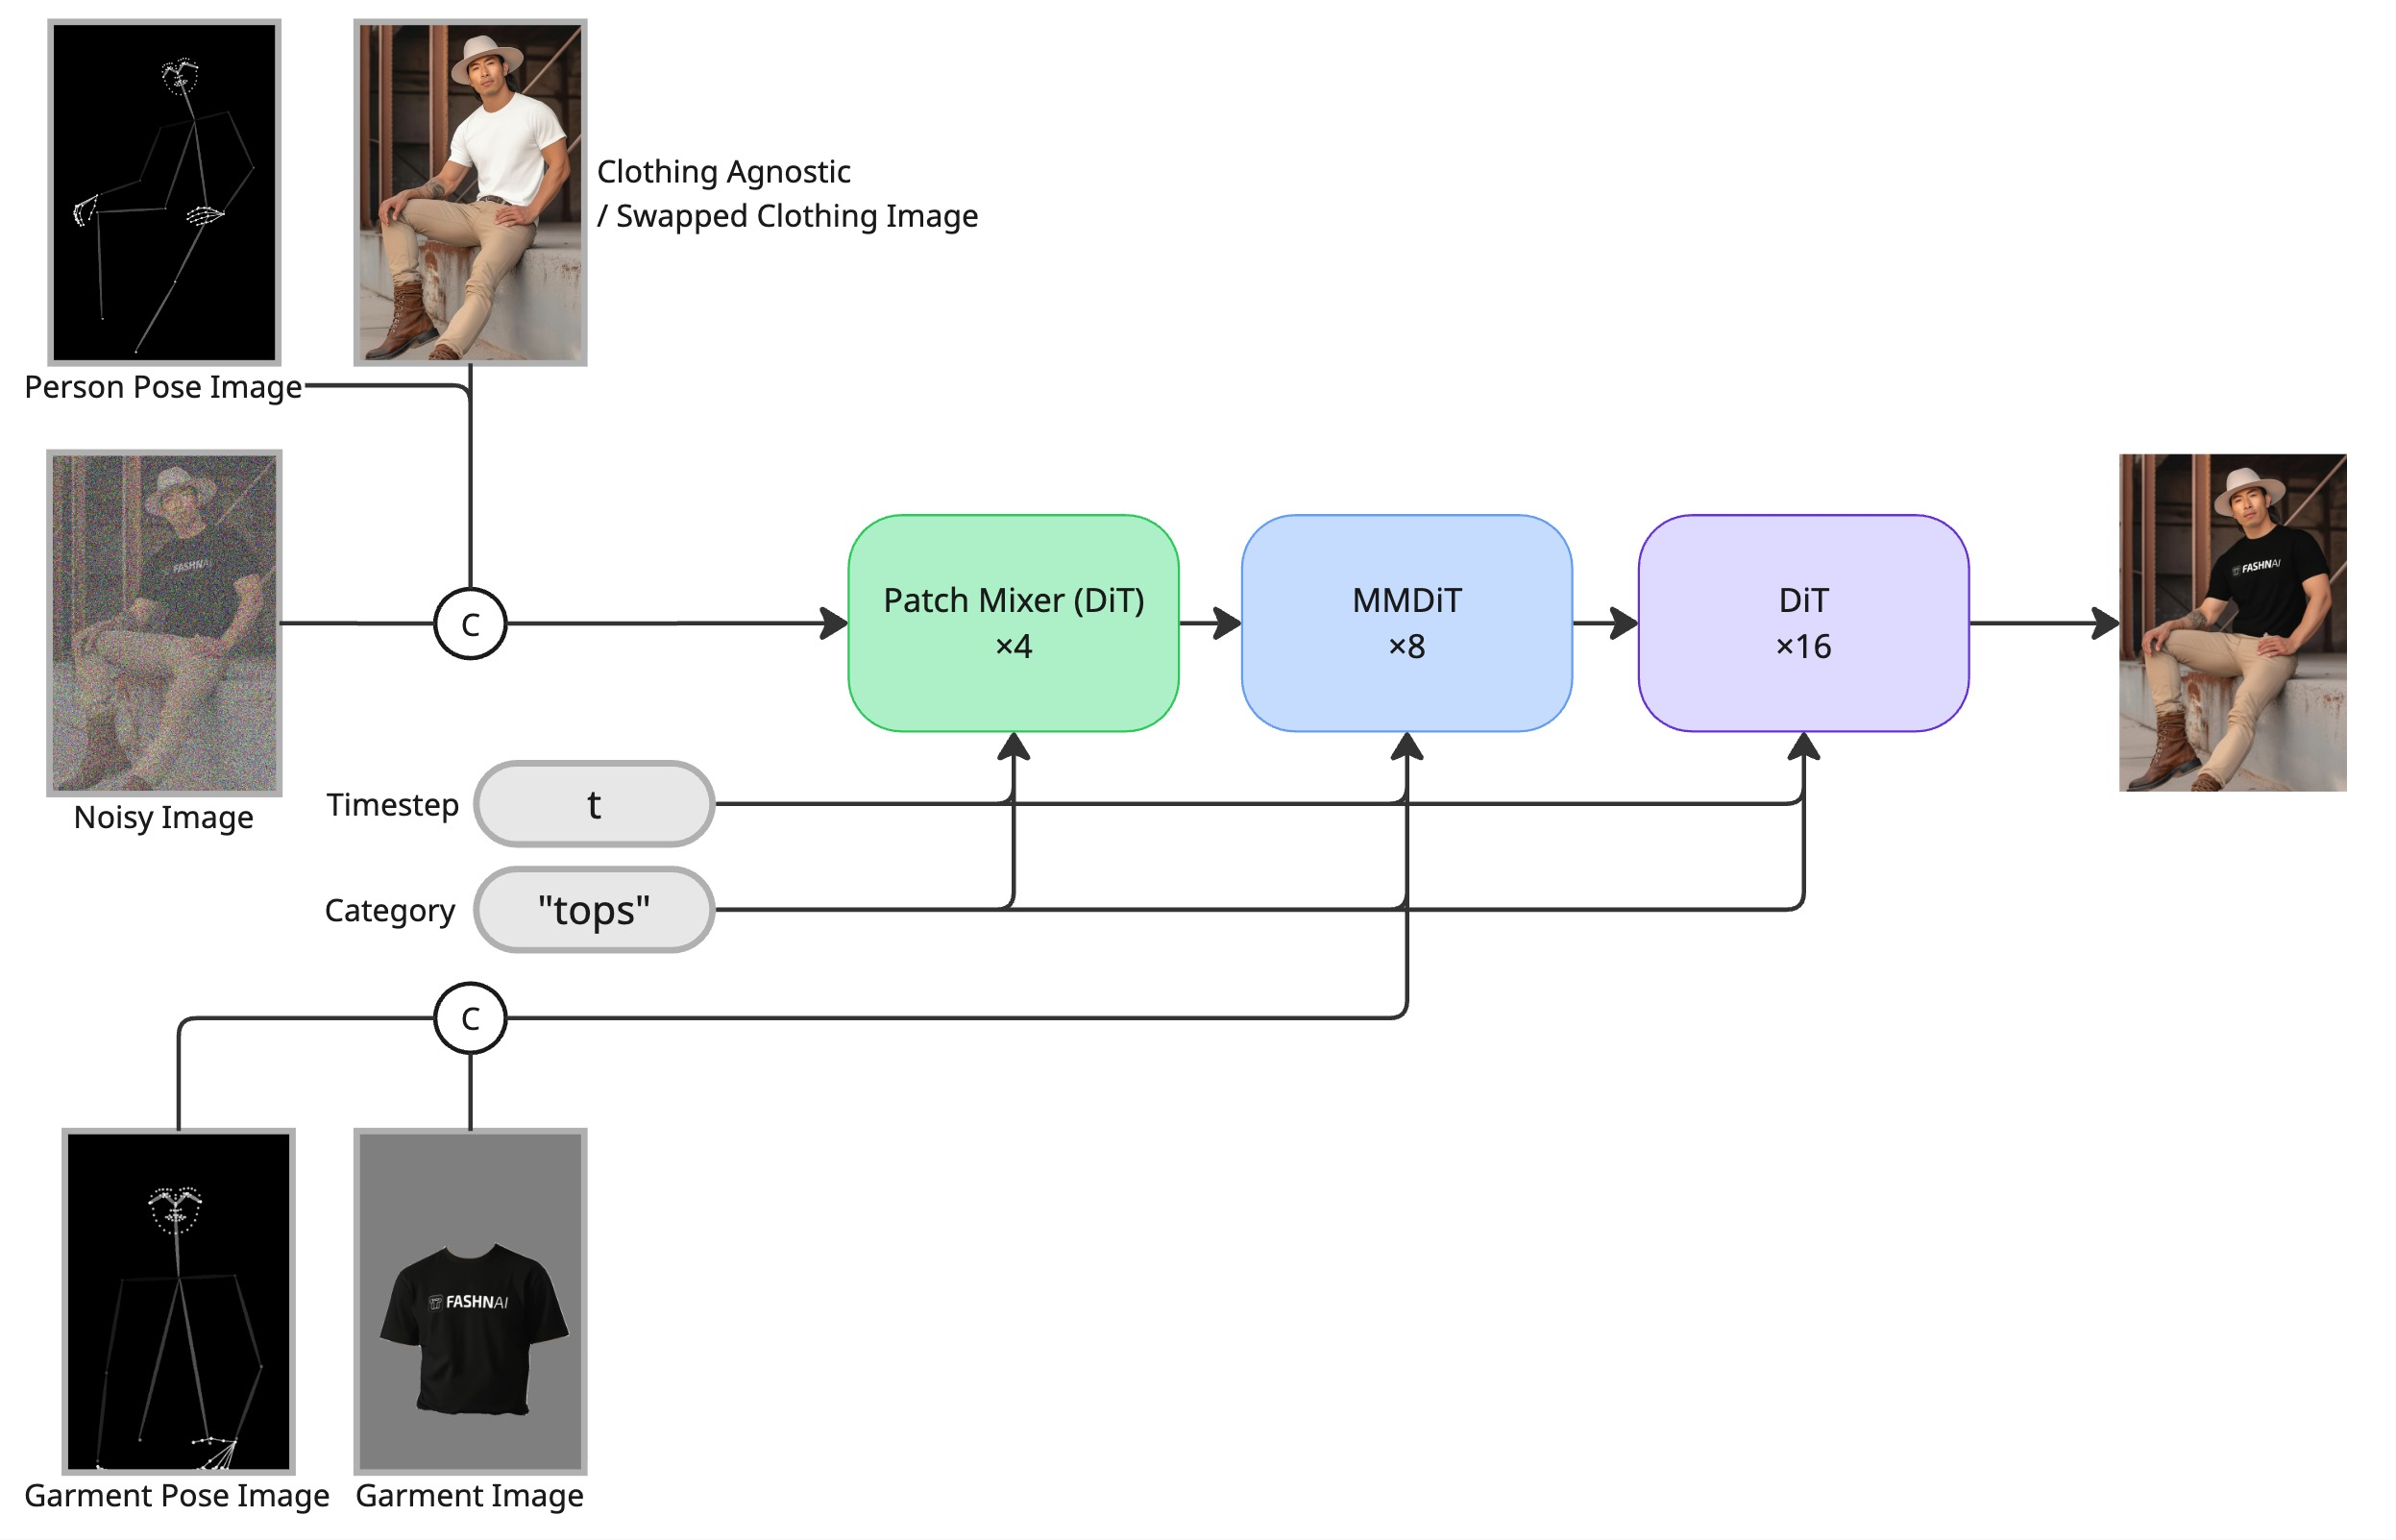
\includegraphics[width=\linewidth]{fashn-vton-diagram.jpg}
  \caption[FASHN VTON v1.5 model flow]{FASHN VTON v1.5 model flow. Pose and garment conditioning, timestep, and category information pass through Patch Mixer, MMDiT, and DiT blocks before producing the final try-on image. Source: FASHN VTON v1.5 research page.}
\end{figure}

The FASHN router is the abstraction boundary:

\begin{itemize}
  \item Reads the configured GPU assignment.
  \item Creates one worker definition per configured GPU.
  \item Pins each worker to a specific CUDA device.
  \item Uses Unix sockets by default to avoid public worker ports.
  \item Performs readiness checks.
  \item Routes requests through least-inflight plus round-robin behavior.
  \item Exports Prometheus metrics with \code{worker_id}, \code{gpu_id}, \code{gpu_uuid}, and \code{status} labels.
  \item Writes structured router and worker logs.
\end{itemize}

\section{VTON Job Lifecycle}

\begin{enumerate}
  \item User uploads the person image and garment image.
  \item API normalizes and stores the image artifacts.
  \item User submits a VTON job.
  \item API checks payload, auth, quota, and workspace concurrency.
  \item The VTON job queue persists a job snapshot.
  \item Runner calls the VTON inference implementation.
  \item Adapter calls the configured FASHN router endpoint.
  \item FASHN worker generates output PNG and report metadata.
  \item API persists request record and job result.
  \item UI polls job status and opens the output artifact.
\end{enumerate}

\begin{center}
\begin{tabular}{ll}
\toprule
\textbf{Status} & \textbf{Meaning} \\
\midrule
accepted & API accepted the job \\
queued & Job is waiting in the queue \\
running & Job is executing \\
completed & Job has an output artifact \\
failed & Job failed and has an error message \\
\bottomrule
\end{tabular}
\end{center}

\section{Multi-GPU Worker Configuration}

In a multi-GPU deployment, the router is configured with the GPU identifiers that it may use. Each worker is assigned to one GPU and communicates over private internal endpoints. The product API continues to call only the router, while Prometheus and Grafana observe worker behavior through labels such as worker identity, GPU identity, request status, latency, and in-flight count.

\begin{center}
\begin{tabular}{lll}
\toprule
\textbf{Worker} & \textbf{CUDA pin} & \textbf{Private endpoint} \\
\midrule
\code{fashn-gpu0} & \code{CUDA_VISIBLE_DEVICES=0} & Unix socket \\
\code{fashn-gpu1} & \code{CUDA_VISIBLE_DEVICES=1} & Unix socket \\
\code{fashn-gpu2} & \code{CUDA_VISIBLE_DEVICES=2} & Unix socket \\
\bottomrule
\end{tabular}
\end{center}

The API and Prometheus do not need to know the private worker endpoints. They talk to the router. Grafana can still display per-worker activity because the router emits worker and GPU labels.

\section{Production LLM Serving}

LLM serving uses an OpenAI-compatible adapter. The adapter calls the chat-completions interface and records:

\begin{itemize}
  \item model name,
  \item provider/base URL after sanitization,
  \item input and output token counts,
  \item latency,
  \item tokens per second,
  \item estimated cost when configured,
  \item guardrail flags,
  \item structured output validation where requested.
\end{itemize}

When the endpoint is unreachable or returns an invalid response, the error is surfaced. That is the correct production behavior.

% ---------------------------------------------------------------------------
\chapter{Governance, Security, and Responsible AI}
% ---------------------------------------------------------------------------

\section{Authentication and Workspace Model}

TryOps uses Keycloak as the OIDC identity provider. The browser authenticates through an authorization-code flow with PKCE. The gateway validates tokens and forwards principal metadata to the backend. On first login, the backend bootstraps a workspace account in Postgres.

\screenshotfig{screenshots/keycloak.png}{Keycloak session control and identity surface}

\section{Quota and Admission Control}

Quota is enforced at two levels:

\begin{itemize}
  \item The Rust gateway performs edge quota/rate admission.
  \item The FastAPI backend enforces workload-level VTON workspace concurrency.
\end{itemize}

\begin{center}
\begin{tabular}{lr}
\toprule
\textbf{Plan} & \textbf{Active VTON jobs} \\
\midrule
free & 1 \\
team & 2 \\
enterprise & 4 \\
\bottomrule
\end{tabular}
\end{center}

Plan limits are different from GPU worker count. A workspace may be limited to one active job even when the router has multiple GPU workers.

\section{Guardrails}

Guardrails run at gateway and API boundaries:

\begin{itemize}
  \item Prompt injection detection.
  \item System prompt leakage prevention.
  \item PII and secret-like string masking.
  \item Output size and structured output validation.
  \item Metrics grouped by risk category.
\end{itemize}

The Go guardrail service is called by the gateway and API through configured internal service URLs.

\section{Promotion Gate}

Model promotion requires:

\begin{itemize}
  \item model card,
  \item data card,
  \item evaluation report,
  \item SBOM,
  \item model artifact scan,
  \item provenance attestation,
  \item risk controls,
  \item owner approvals,
  \item policy verdict.
\end{itemize}

\begin{center}
\begin{tabular}{ll}
\toprule
\textbf{State} & \textbf{Meaning} \\
\midrule
candidate & Produced by pipeline, not trusted yet \\
challenger & Passed staging gate, eligible for shadow/canary \\
champion & Current promoted model \\
rejected & Blocked by policy \\
archived & Kept for audit and rollback history \\
\bottomrule
\end{tabular}
\end{center}

\section{Supply Chain and Privacy}

The repository contains supply-chain and model-source documentation for model origin, dependency inventory, dataset licensing, and promotion decisions. Production logs should not contain raw prompts, raw uploaded images, or provider secrets. Logs should reference artifacts, request IDs, trace IDs, and job IDs instead.

% ---------------------------------------------------------------------------
\chapter{Observability and Operations}
% ---------------------------------------------------------------------------

\section{Dashboards}

\begin{longtable}{p{5cm}p{9.8cm}}
\toprule
\textbf{Dashboard} & \textbf{Purpose} \\
\midrule
TryOps Service Overview & Request rate, error ratio, latency, memory, queue depth, gateway errors \\
TryOps Model Quality & Quality score, VTON latency, LLM throughput, completed inference \\
TryOps Cost and Capacity & Cost, quota utilization, cache hit rate, energy/carbon \\
TryOps Guardrails & Blocked/redacted/reviewed findings by OWASP-style risk category \\
TryOps Observability Drilldown & Logs, job lifecycle, FASHN service logs, OTel/Tempo/Loki health \\
\bottomrule
\end{longtable}

\section{Logs}

Useful log categories:

\begin{itemize}
  \item API request and job lifecycle events.
  \item FASHN router events.
  \item Per-worker VTON inference events.
  \item Model-serving process logs.
  \item Trace spans for API and background jobs.
\end{itemize}

Grafana should make these logs searchable by job identifier, request identifier, account identifier, worker identifier, and GPU identifier. This is necessary to debug cases where the UI is waiting but the backend has completed or failed a job.

\section{Metrics}

Important metric groups:

\begin{itemize}
  \item HTTP request count and duration by service and status.
  \item VTON job lifecycle counters and active queue depth.
  \item FASHN router worker requests and in-flight counts.
  \item Per-worker latency and failure count.
  \item LLM token throughput, latency, and error rate.
  \item Guardrail block/redaction counters.
  \item Quota admission and remaining capacity.
  \item Hardware usage from host exporters and GPU exporters.
\end{itemize}

\section{Developer-Local Ports}

Figure~\ref{fig:port-service-diagram} separates three concerns: host ports exposed during local development, private Compose-network endpoints, and host-side inference endpoints used by GPU-serving processes.

\clearpage
\begin{figure}[p]
\centering
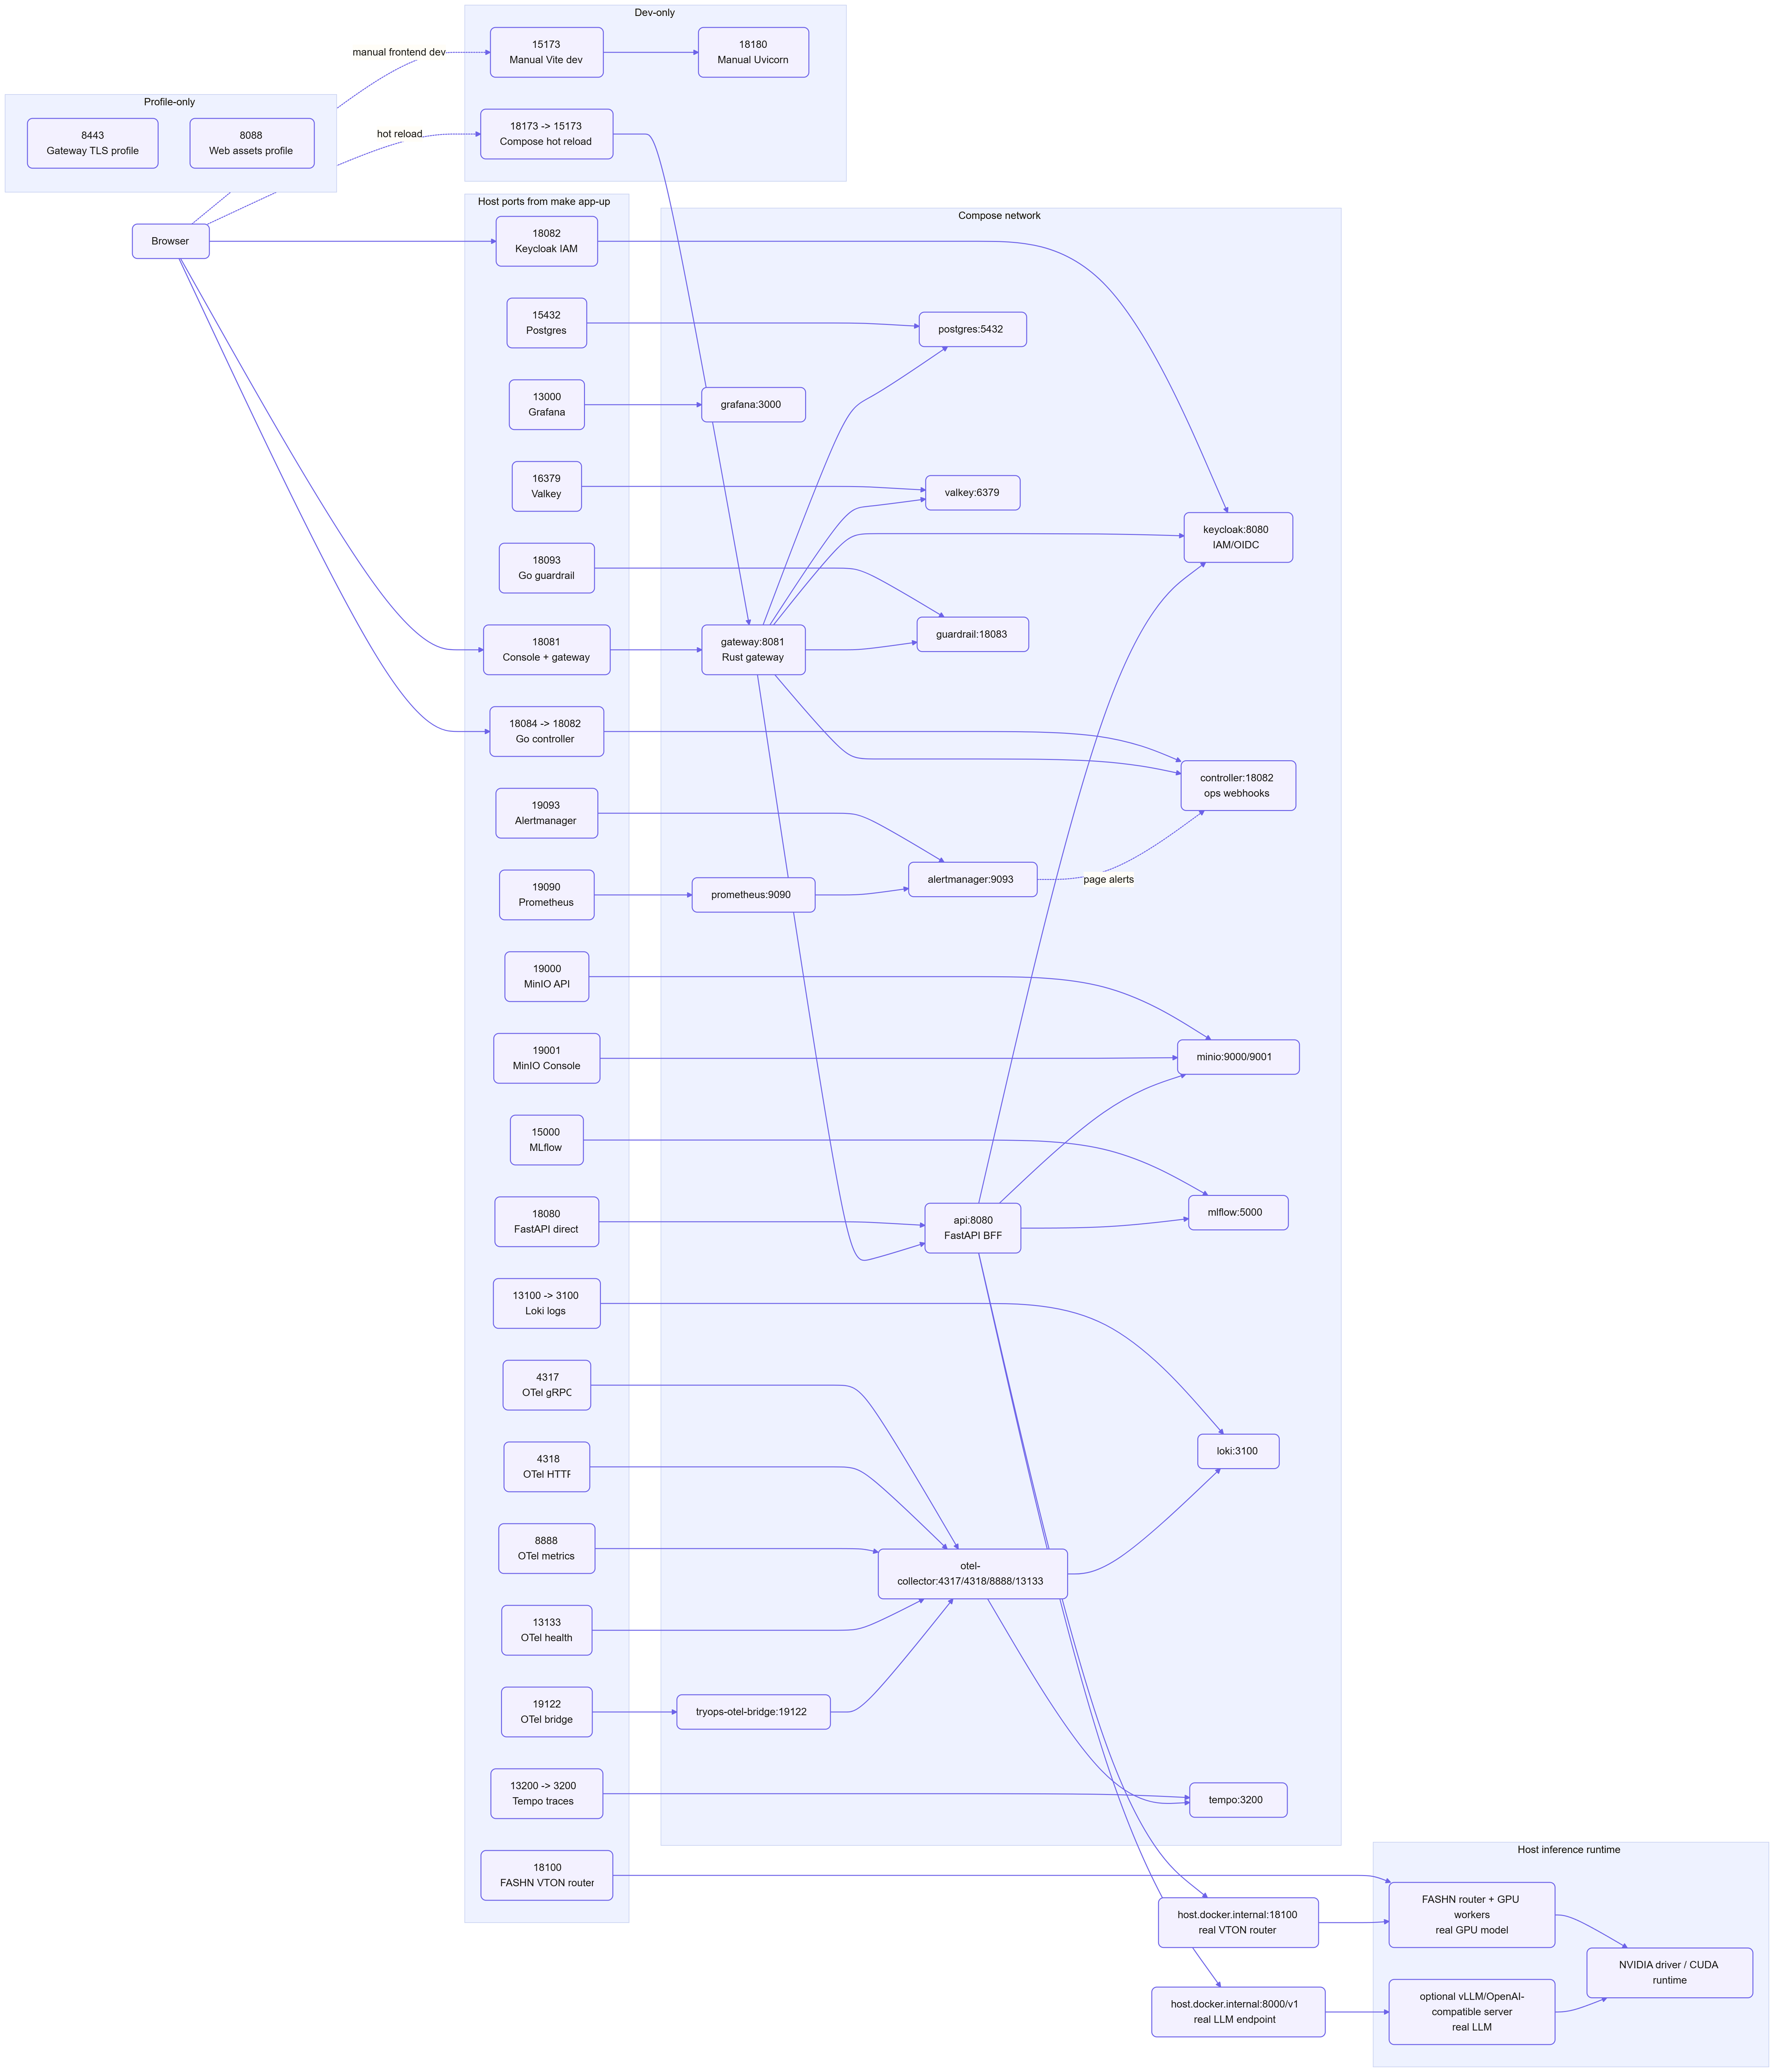
\includegraphics[width=\linewidth,height=0.88\textheight,keepaspectratio]{port-service-diagram.png}
\caption{Developer-local service and port topology.}
\label{fig:port-service-diagram}
\end{figure}
\clearpage

\begingroup
\scriptsize
\setlength{\tabcolsep}{2.5pt}
\renewcommand{\arraystretch}{1.16}
\begin{longtable}{>{\raggedright\arraybackslash}p{3.35cm}>{\raggedright\arraybackslash}p{1.25cm}>{\raggedright\arraybackslash}p{3.95cm}>{\raggedright\arraybackslash}p{6.35cm}}
\caption{Developer-local \code{make app-up} ports and override variables.}
\label{tab:developer-local-ports}\\
\toprule
\textbf{Service} & \textbf{Port} & \textbf{Override variable} & \textbf{Notes} \\
\midrule
\endfirsthead
\toprule
\textbf{Service} & \textbf{Port} & \textbf{Override variable} & \textbf{Notes} \\
\midrule
\endhead
TryOps Console + Rust gateway & \code{18081} & \code{TRYOPS_GATEWAY_PORT} & Main app URL. Use this entry point first. \\
FastAPI backend direct & \code{18080} & \code{TRYOPS_API_PORT} & Direct API/docs access. The gateway normally proxies this service. \\
Keycloak IAM & \code{18082} & \code{TRYOPS_KEYCLOAK_PORT} & OIDC/IAM service. Container port is \code{8080}. \\
Go controller & \code{18084} & \code{TRYOPS_CONTROLLER_PORT} & Webhook/control-plane service. Container port is \code{18082}; Alertmanager calls \code{controller:18082/alerts/webhook} inside Compose. \\
FASHN VTON router & \code{18100} & \code{FASHN_VTON_ROUTER_PORT} & Host-side production-local VTON router started by \code{make app-up}. The API reaches it through \code{host.docker.internal:18100}. \\
FASHN VTON single-worker debug & \code{18101} & \code{FASHN_VTON_PORT} & Optional direct service for isolated debugging with \code{make fashn-vton-service-bg}. \code{make app-up} does not use it. \\
Optional local vLLM/OpenAI-compatible LLM & \code{8000} & \code{VLLM_PORT}\newline\code{VLLM_BASE_URL}\newline\code{TRYOPS_LLM_BASE_URL} & Host-side LLM endpoint for self-hosted vLLM. If \code{TRYOPS_LLM_BASE_URL} points to an external OpenAI-compatible provider, no local LLM port is needed. \\
Postgres & \code{15432} & \code{TRYOPS_POSTGRES_PORT} & Database for the full Compose stack. \\
Valkey & \code{16379} & \code{TRYOPS_VALKEY_PORT} & Hot quota and rate-counter store. \\
MinIO API & \code{19000} & \code{TRYOPS_MINIO_PORT} & Object and artifact storage API. \\
MinIO Console & \code{19001} & \code{TRYOPS_MINIO_CONSOLE_PORT} & Browser UI for MinIO. \\
MLflow & \code{15000} & \code{TRYOPS_MLFLOW_PORT} & Experiment and model tracking. \\
Prometheus & \code{19090} & \code{TRYOPS_PROMETHEUS_PORT} & Metrics database. \\
Alertmanager & \code{19093} & \code{TRYOPS_ALERTMANAGER_PORT} & Alert routing. \\
Grafana & \code{13000} & \code{TRYOPS_GRAFANA_PORT} & Dashboards. Fresh local volume defaults to \code{admin} / \code{admin}. \\
Loki & \code{13100} & \code{TRYOPS_LOKI_PORT} & Log store used by Grafana when observability is enabled. Container port is \code{3100}. \\
Tempo & \code{13200} & \code{TRYOPS_TEMPO_PORT} & Trace store used by Grafana when observability is enabled. Container port is \code{3200}. \\
Go guardrail sidecar & \code{18093} & \code{TRYOPS_GUARDRAIL_PORT} & LLM guardrail service. Usually called by gateway/API. Container port is \code{18083}. \\
OpenTelemetry gRPC & \code{4317} & \code{TRYOPS_OTEL_GRPC_PORT} & OTLP gRPC receiver. \\
OpenTelemetry HTTP & \code{4318} & \code{TRYOPS_OTEL_HTTP_PORT} & OTLP HTTP receiver. \\
OpenTelemetry metrics & \code{8888} & \code{TRYOPS_OTEL_METRICS_PORT} & Collector metrics endpoint. \\
OpenTelemetry health & \code{13133} & \code{TRYOPS_OTEL_HEALTH_PORT} & Collector health endpoint. \\
OTel bridge metrics & \code{19122} & \code{TRYOPS_OTEL_BRIDGE_PORT} & Metrics endpoint path is \code{/metrics}. Bridges local TryOps JSONL logs/traces into OTLP for Grafana, Loki, and Tempo. \\
\bottomrule
\end{longtable}
\endgroup
\clearpage

For a shared data center, this broad developer-local port surface should be replaced by a smaller ingress surface: gateway, Keycloak, and admin-restricted Grafana. Databases, object stores, metrics stores, guardrail, and model endpoints should remain private.

\section{Deployment Preconditions}

A production-facing deployment must be configured with model endpoints, secured provider credentials, disabled development shortcuts, and explicit GPU readiness checks for VTON inference. Operational checks should verify service health, authentication, quota admission, object storage, observability, and model-serving readiness before users are allowed to submit expensive inference jobs.

% ---------------------------------------------------------------------------
\chapter{Experiments and Evaluation}
% ---------------------------------------------------------------------------

\section{VTON Benchmark Results}

\begin{center}
\metriccard[TryOpsTeal]{0.29\linewidth}{Best quality score}{0.888121 SSIM}
\hfill
\metriccard[TryOpsTeal]{0.29\linewidth}{Best image fidelity}{18.915 PSNR}
\hfill
\metriccard[TryOpsTeal]{0.29\linewidth}{Lowest VTON memory}{4.825 GB VRAM}

\vspace{0.45em}

\metriccard[TryOpsBlue]{0.43\linewidth}{Fastest average latency}{17,842.30 ms}
\hfill
\metriccard[TryOpsBlue]{0.43\linewidth}{Highest VTON throughput}{0.054261 req/s}
\end{center}

\begin{table}[H]
\centering
\caption{Detailed VTON benchmark results used for model selection.}
\label{tab:vton-benchmark}
\renewcommand{\arraystretch}{1.22}
\small
\resizebox{\linewidth}{!}{%
\begin{tabular}{lrrrrrrrr}
\toprule
\textbf{Candidate} & \textbf{SSIM} & \textbf{PSNR} & \textbf{Avg ms} & \textbf{P95 ms} & \textbf{req/s} & \textbf{Model ms} & \textbf{GPU \%} & \textbf{VRAM GB} \\
\midrule
\textbf{FASHN VTON v1.5} & \metric[TryOpsTeal]{0.888121} & \metric[TryOpsTeal]{18.915} & 21,337.50 & 23,244.00 & 0.045439 & 19,969.60 & \metric[TryOpsGold]{100.00} & \metric[TryOpsTeal]{4.825} \\
CatVTON & 0.861734 & 18.284 & \metric[TryOpsBlue]{17,842.30} & \metric[TryOpsBlue]{19,604.00} & \metric[TryOpsBlue]{0.054261} & \metric[TryOpsBlue]{16,512.80} & 96.50 & 6.742 \\
IDM-VTON & 0.879462 & 18.671 & 42,586.70 & 47,918.00 & 0.022751 & 40,318.40 & 99.20 & 13.684 \\
OOTDiffusion & 0.852918 & 17.936 & 35,214.90 & 39,876.00 & 0.027502 & 33,087.60 & 98.40 & 10.927 \\
\bottomrule
\end{tabular}%
}

\vspace{0.45em}
\begin{minipage}{0.94\linewidth}
\footnotesize
\textbf{Selection reading.} FASHN VTON v1.5 is the strongest quality-first candidate in this run because it has the best SSIM, best PSNR, and lowest VRAM usage. CatVTON is the strongest latency-first candidate, but its recorded quality metrics are lower.
\end{minipage}
\end{table}

\begin{figure}[H]
\centering
\small
\begin{tabularx}{\linewidth}{>{\raggedright\arraybackslash}X>{\raggedright\arraybackslash}X>{\raggedright\arraybackslash}X}
\toprule
\textbf{Best quality} & \textbf{Best latency} & \textbf{Heavier comparison candidates} \\
\midrule
FASHN VTON v1.5 leads SSIM and PSNR in the recorded run while using the least GPU memory. &
CatVTON has the lowest average latency, P95 latency, and model latency with the highest throughput. &
IDM-VTON and OOTDiffusion cost more latency, VRAM, and host RAM in this benchmark. \\
\bottomrule
\end{tabularx}

\vspace{0.6em}
\scriptsize
\resizebox{0.92\linewidth}{!}{%
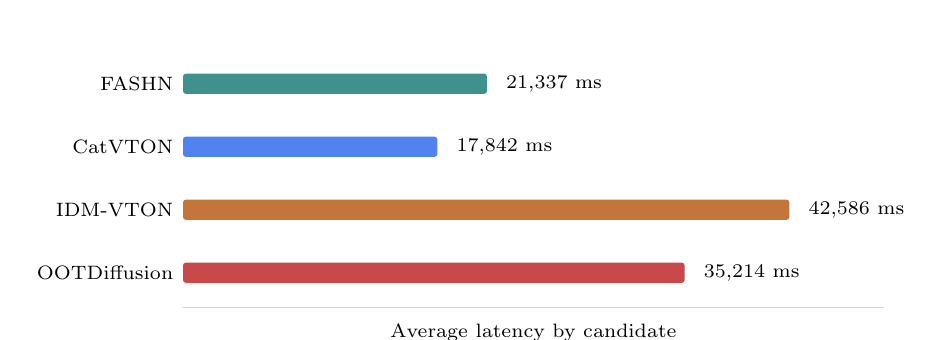
\begin{tikzpicture}[
  x=1cm,
  y=0.80cm,
  every node/.style={font=\scriptsize},
  bar/.style={draw=none, rounded corners=1pt}
]
\node[anchor=east] at (0,3) {FASHN};
\fill[bar, TryOpsTeal!80] (0,2.84) rectangle (3.86,3.16);
\node[anchor=west] at (3.98,3) {21,337 ms};

\node[anchor=east] at (0,2) {CatVTON};
\fill[bar, TryOpsBlue!80] (0,1.84) rectangle (3.23,2.16);
\node[anchor=west] at (3.35,2) {17,842 ms};

\node[anchor=east] at (0,1) {IDM-VTON};
\fill[bar, TryOpsGold!80] (0,0.84) rectangle (7.70,1.16);
\node[anchor=west] at (7.82,1) {42,586 ms};

\node[anchor=east] at (0,0) {OOTDiffusion};
\fill[bar, TryOpsRed!80] (0,-0.16) rectangle (6.37,0.16);
\node[anchor=west] at (6.49,0) {35,214 ms};

\draw[TryOpsLine] (0,-0.55) -- (8.90,-0.55);
\node[anchor=north] at (4.45,-0.66) {Average latency by candidate};
\end{tikzpicture}%
}
\caption{VTON benchmark interpretation and average latency comparison.}
\end{figure}

Interpretation:

\begin{itemize}
  \item FASHN VTON v1.5 leads SSIM and PSNR in the recorded table and uses the least GPU memory.
  \item CatVTON has the best latency/throughput but lower recorded quality.
  \item IDM-VTON and OOTDiffusion consume more latency, VRAM, and host RAM.
  \item FASHN is a reasonable production-local target for a quality-first product path.
\end{itemize}

\section{LLM Optimization Results}

The LLM optimization summary records a Pareto frontier:

\begin{table}[H]
\centering
\caption{Highlighted LLM optimization measurements.}
\small
\begin{tabularx}{\linewidth}{>{\bfseries}p{2.2cm}p{3.1cm}p{3.1cm}X}
\toprule
\textbf{Mode} & \textbf{VRAM} & \textbf{Decode speed} & \textbf{Reading} \\
\midrule
fp16 & \metric[TryOpsBlue]{1.010 GB} & \metric[TryOpsTeal]{27.4 tokens/s} & Fastest measured decode speed. \\
8-bit & \metric[TryOpsGold]{0.647 GB} & \metric[TryOpsRed]{5.9 tokens/s} & Lower memory than fp16, but slower in this recorded run. \\
4-bit & \metric[TryOpsTeal]{0.478 GB} & \metric[TryOpsBlue]{13.9 tokens/s} & Recommended low-memory option in this comparison. \\
\bottomrule
\end{tabularx}
\end{table}

The engineering lesson is that lower precision does not automatically mean lower total cost or energy. If a quantized model decodes much slower at similar board power, joules per token and rental cost per million tokens may increase.

\section{Native Boundary Evaluation}

Benchmark results report that the Go load driver measured Rust \code{/health} at \metric[TryOpsTeal]{24,840.8 requests/s} versus FastAPI at \metric[TryOpsGold]{1,539.4 requests/s} on the same machine, a throughput difference of about \metric[TryOpsBlue]{16.1x}. This does not mean Python is removed. It means Python remains the ML workflow layer while Rust/Go/C++ support the edge, control plane, and native tooling.

\section{Balancer Testing}

The expected multi-GPU router test sends concurrent requests to the router and verifies that completed-request counters increase across multiple worker and GPU labels. If only one GPU receives all work, the first things to check are workspace job concurrency, API job worker count, router worker readiness, GPU assignment, and whether the test sends enough simultaneous jobs to exceed one worker's in-flight capacity.

% ---------------------------------------------------------------------------
\chapter{Limitations and Future Work}
% ---------------------------------------------------------------------------

\section{Current Limitations}

\begin{itemize}
  \item Full vLLM live benchmark depends on the active host environment and installed serving runtime.
  \item Production KServe/Kubeflow cluster deployment is a target profile, not the currently packaged local stack.
  \item Representative human evaluation panels for VTON quality and fairness remain future work.
  \item Over-quantizing the VTON model can produce blurred garments, lost texture, and visually invalid try-on outputs; quantized VTON deployment must be gated by image-quality regression tests instead of only API success checks.
  \item Some UI operator workflows need additional click-through detail and export features.
  \item Shared-datacenter port reduction should be completed by moving internal services behind ingress/private networks.
  \item GPU utilization dashboards require host GPU exporters and per-worker router metrics to be consistently scraped.
  \item Active VTON jobs must remain visible after browser refresh while queued or running; this is essential for trustworthy handling of expensive GPU work.
\end{itemize}

One concrete VTON limitation observed during optimization is that aggressive quantization or overly compressed runtime settings can preserve API success while reducing visual quality. The output may become blurred around garment and body regions, with weak texture transfer and degraded person boundaries. This means VTON promotion cannot rely only on HTTP success, latency, and GPU memory; it also needs image-quality regression checks.

\begin{figure}[H]
  \centering
  
\includegraphics[width=0.42\linewidth]{blur_vton.png}
  \caption[VTON over-quantization limitation]{VTON over-quantization limitation: reduced runtime cost can produce blurred garment and body regions, so optimized variants require visual quality gates before promotion.}
\end{figure}

\section{Future Work}

\begin{enumerate}
  \item Finish active job persistence and refresh-safe UI behavior.
  \item Harden shared-host deployment with a minimal public port surface.
  \item Add host GPU exporter integration and Grafana GPU worker dashboards.
  \item Add a production secret manager integration.
  \item Expand VTON evaluation with human preference labels and fairness slices.
  \item Add broader LLM provider/model compatibility tests.
  \item Package a KServe/Kubeflow profile for cluster-grade deployment.
  \item Improve incident response runbooks and dashboard drilldowns.
\end{enumerate}

\section{Implementation Boundary}

The strongest position for this project is to be explicit:

\begin{itemize}
  \item Implemented paths: Rust gateway, FastAPI backend, Keycloak, MinIO, MLflow, Prometheus/Grafana/Loki/Tempo, FASHN VTON router, OpenAI-compatible LLM adapter.
  \item Local/conditional paths: vLLM live benchmark and GPU exporter availability depend on host runtime.
  \item Test/evaluation paths: seeded examples and offline evaluation fixtures.
  \item Future paths: full cluster deployment, larger fairness panels, production-grade external secret handling.
\end{itemize}

This separation makes the project more defensible, not less. It prevents overclaiming and gives operators a clear list of what is production-ready versus what still needs hardening.

% ---------------------------------------------------------------------------
\chapter{Conclusion}
% ---------------------------------------------------------------------------

TryOps demonstrates an MLOps platform that treats models as governed production assets rather than isolated notebook outputs. The project integrates a usable product console, model-serving boundaries, account and quota control, artifact storage, model governance, observability, native control-plane components, and explicit production readiness checks.

The most important result is architectural: VTON and LLM workloads can share the same operational spine while preserving workload-specific needs. VTON requires GPU-aware job control, image artifact lineage, and visual quality assessment. LLM serving requires token accounting, endpoint health, guardrails, and latency/cost measurements. TryOps uses the same gateway, API, observability, storage, and governance foundation for both.

The project still has work to do before it can be treated as a hardened multi-tenant data-center platform. However, its current design and repository artifacts already show the core MLOps contribution: production model paths are separated from diagnostics, model changes must earn promotion, and operators can inspect the records needed to debug, govern, and roll back the system.

% ---------------------------------------------------------------------------
\chapter*{References}
\addcontentsline{toc}{chapter}{References}
% ---------------------------------------------------------------------------

\begin{thebibliography}{99}

\bibitem{opentelemetry}
OpenTelemetry, ``OpenTelemetry Documentation,'' [Online]. Available:
\url{https://opentelemetry.io/docs/}. Accessed: July 4, 2026.

\bibitem{prometheus}
Prometheus Authors, ``Prometheus Documentation,'' [Online]. Available:
\url{https://prometheus.io/docs/}. Accessed: July 4, 2026.

\bibitem{grafana}
Grafana Labs, ``Grafana Documentation,'' [Online]. Available:
\url{https://grafana.com/docs/grafana/latest/}. Accessed: July 4, 2026.

\bibitem{mlflow}
MLflow, ``MLflow Documentation,'' [Online]. Available:
\url{https://mlflow.org/docs/latest/}. Accessed: July 4, 2026.

\bibitem{minio}
MinIO, ``MinIO Object Storage Documentation,'' [Online]. Available:
\url{https://min.io/docs/minio/linux/}. Accessed: July 4, 2026.

\bibitem{keycloak}
Keycloak, ``Keycloak Documentation,'' [Online]. Available:
\url{https://www.keycloak.org/documentation}. Accessed: July 4, 2026.

\bibitem{fashn-vton}
FASHN, ``FASHN VTON 1.5 Research,'' [Online]. Available:
\url{https://fashn.ai/research/vton-1-5}. Accessed: July 4, 2026.

\bibitem{vllm}
vLLM Project, ``vLLM Documentation,'' [Online]. Available:
\url{https://docs.vllm.ai/}. Accessed: July 4, 2026.

\bibitem{nist-ai-rmf}
National Institute of Standards and Technology, ``Artificial Intelligence Risk
Management Framework,'' [Online]. Available:
\url{https://www.nist.gov/itl/ai-risk-management-framework}. Accessed:
July 4, 2026.

\bibitem{owasp-llm}
OWASP Foundation, ``OWASP Top 10 for Large Language Model Applications,''
[Online]. Available:
\url{https://owasp.org/www-project-top-10-for-large-language-model-applications/}.
Accessed: July 4, 2026.

\bibitem{slsa}
OpenSSF, ``Supply-chain Levels for Software Artifacts,'' [Online]. Available:
\url{https://slsa.dev/}. Accessed: July 4, 2026.

\bibitem{syft}
Anchore, ``Syft: SBOM Generator,'' [Online]. Available:
\url{https://github.com/anchore/syft}. Accessed: July 4, 2026.

\bibitem{trivy}
Aqua Security, ``Trivy Documentation,'' [Online]. Available:
\url{https://aquasecurity.github.io/trivy/}. Accessed: July 4, 2026.

\bibitem{cosign}
Sigstore, ``Cosign Documentation,'' [Online]. Available:
\url{https://docs.sigstore.dev/cosign/}. Accessed: July 4, 2026.

\end{thebibliography}

\end{document}
